
\subsection{Sample from distributions}
\label{subsec:SampleViaDistribution}

% Intuition
Assuming the distribution $p$ of a variable $x$ is known, i.e. $x \sim p$, it is possible to sample from it.
Sampling can either be done directly or 
via approximation schemes such as rejection sampling and Monte Carlo sampling \citet{robinson_contrastive_2021}.
However, in the context of \ac{cl}, the true data distribution of the different classes is often not available 
due to the nature of unsupervised learning scenarios.
Therefore, some scientists formulate assumptions or simplify the problem.

% mathematical foundation
%Positive pairs ($x$, $x^+$) are considered to originate from the same class.
% Let $\rho(c), c \in \mathcal{C}$ be the distribution over the latent classes and 
% let $h: \mathcal{X} \rightarrow \mathcal{C}$ be the ground truth assigning class labels $c \in \mathcal{C}$ to inputs $x \in \mathcal{X}$.
% Hence, $x \sim x'$ if $h(x) = h(x')$ \citet{robinson_contrastive_2021,chuang_debiased_2020}.

% PU learning
\subsubsection{\ac{pu} approximation}\label{subsec:pu_approximation}

\citet{chuang_debiased_2020} assume a \ac{pu} learning scenario, 
where positive samples and an unlabeled image dataset $p(x)$ are available.
Since positive samples may not be available in reality, 
the positive distribution $p^+$ is mimicked by data augmentations.

\citeauthor{chuang_debiased_2020}'s goal is to sample \acp{tn}.
They denote sampling bias the phenomenon of sampling \acp{fn} as illustrated in \autoref{fig:sampling_bias}a.
When randomly sampling negative samples from the data distribution $p(x)$ 
a negative sample can inherently belong to the same latent class as the anchor.
The negative effect of sampling bias on the model's performance is illustrated in \autoref{fig:sampling_bias}b.
Consequently, they propose a debiased contrastive objective that corrects for sampling \acp{fn} 
%i.e., the selection of negative samples that have the same label as the anchor, 
in an unsupervised scenario.
The idea is to generate positive samples using augmentations,
to sample negative samples $x^-$ from the data distribution $p(x)$
and to add a correction term for \acp{fn} in the loss function.

\begin{figure}%
    \centering
    \subfloat[\centering Visualization of sampling bias similar to \citet{chuang_debiased_2020}. Sampling $x_i^-$ from $p$ can result in \ac{fn}.]
    {{\includegraphics[width=5cm]{images/sampling_bias.png} }}%
    \qquad
    \subfloat[\centering Negative influence of sampling bias on accuracy from \citet{chuang_debiased_2020}.]{{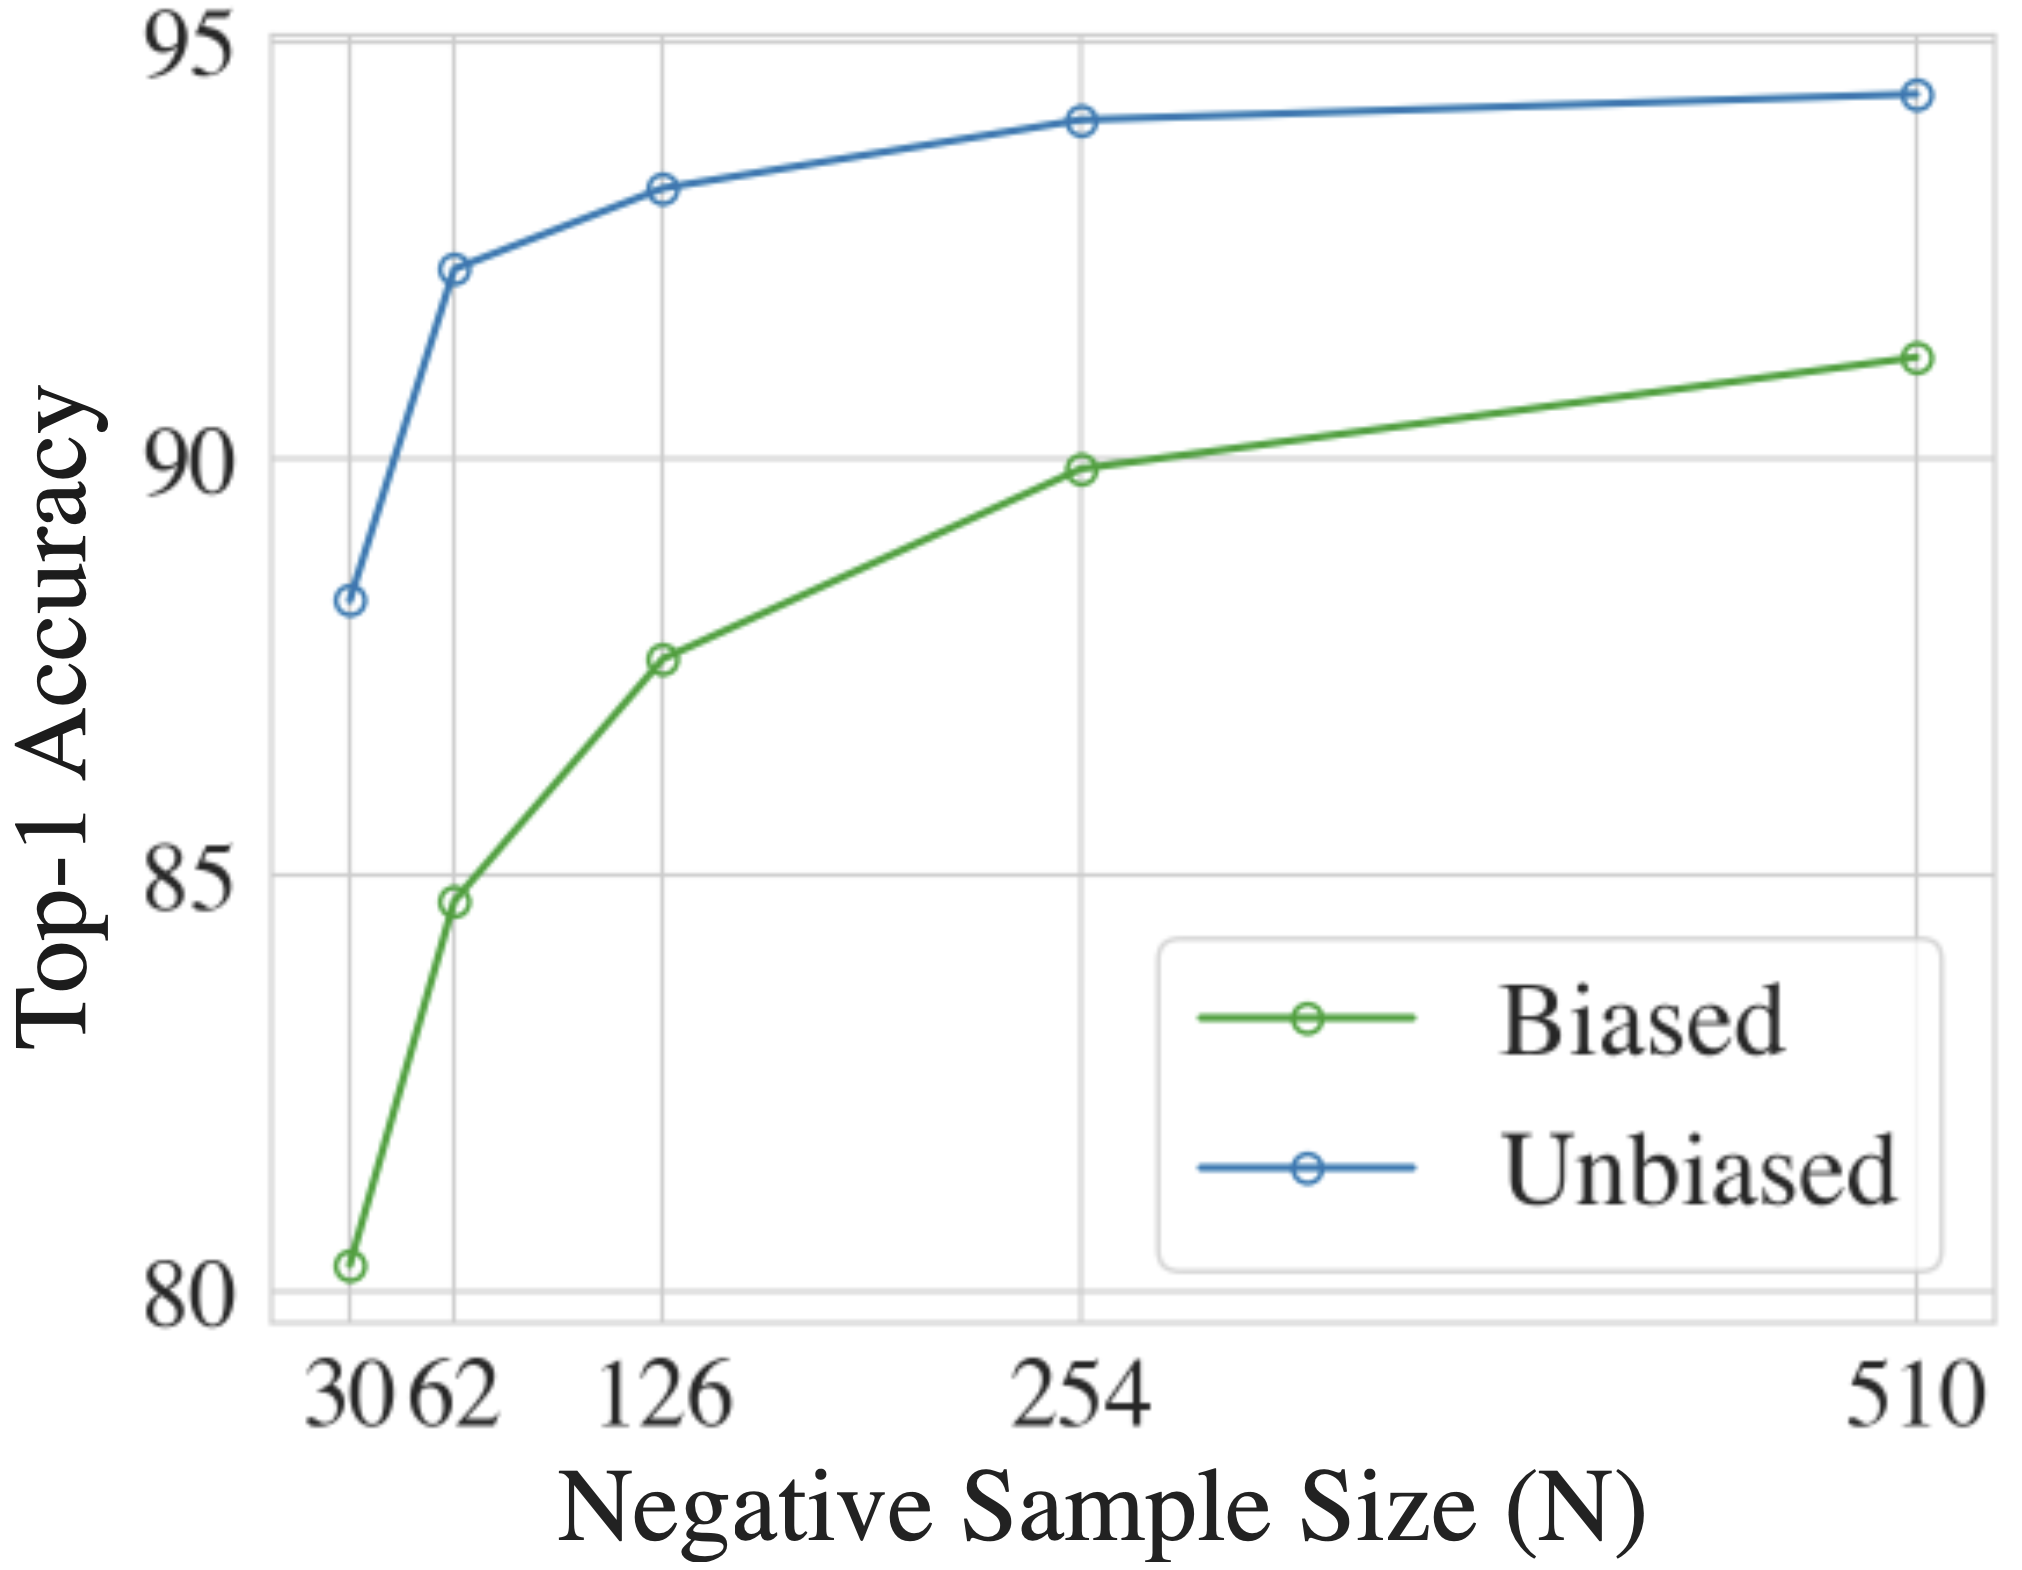
\includegraphics[width=5cm]{images/debiased_sampling_accuracy.png} }}%
    \caption{Visualization of sampling bias and its effect on the model's performance.}%
    \label{fig:sampling_bias}%
\end{figure}


% Choose hardness (Robinson)
\subsubsection{Choosing the hardness of negative samples}\label{subsec:choose_hardness}

\citet{robinson_contrastive_2021} 
extend \citet{chuang_debiased_2020}'s approach to sampling from distributions of image data.
Again, sampling from the positive sample distribution is approximated by sampling from a set of transformations
while negative samples $x^-$ are obtained by sampling from the data distribution $p(x)$.

\citet{robinson_contrastive_2021} introduce the concentration parameter $\beta$ 
to enable user-specific hardness of the negative samples.
$\beta$ is a multiplicative factor for the similarity, i.e. dot product $\beta f(x)^\text{T}f(x^-)$, of two sample feature space representations.
Hence, large values of $\beta$ lead to sampling very hard negative samples and thus, 
increase the risk of sampling \acp{fn}.


% graphs (ProGCL)
\subsubsection{Graphs}\label{subsec:graph_distribution}

Another prominent data structure is graphs, which can model 
social networks, citation networks, or knowledge graphs.
\citet{progcl_2022} propose an approach to mine negative samples for \ac{cl} on graphs called \progcl{}. 
As a motivation, the authors compare the similarity between the anchor and \acp{tn} 
to the similarity between the anchor and \acp{fn} 
across multiple datasets for both conventional \ac{cl} and \ac{gcl}.
The resulting distributions shown in \autoref{fig:sim_t_f_neg_image_graph} 
indicate that for \ac{gcl} the majority of highly similar negative samples are \acp{fn}, 
while for conventional \ac{cl} there seems to be no clear trend.
Moreover, the authors found that both the \ac{tn} and \ac{fn} distributions are best modeled by a beta mixture model %\acl{bmm} 
since it is able to fit the skewed empirical distribution.
The distribution is fitted using the \ac{em} algorithm on a subset of samples for a reduction of computational costs.

\begin{figure}%
    \centering
    \subfloat[\centering CIFAR-10 (Image)]
    {{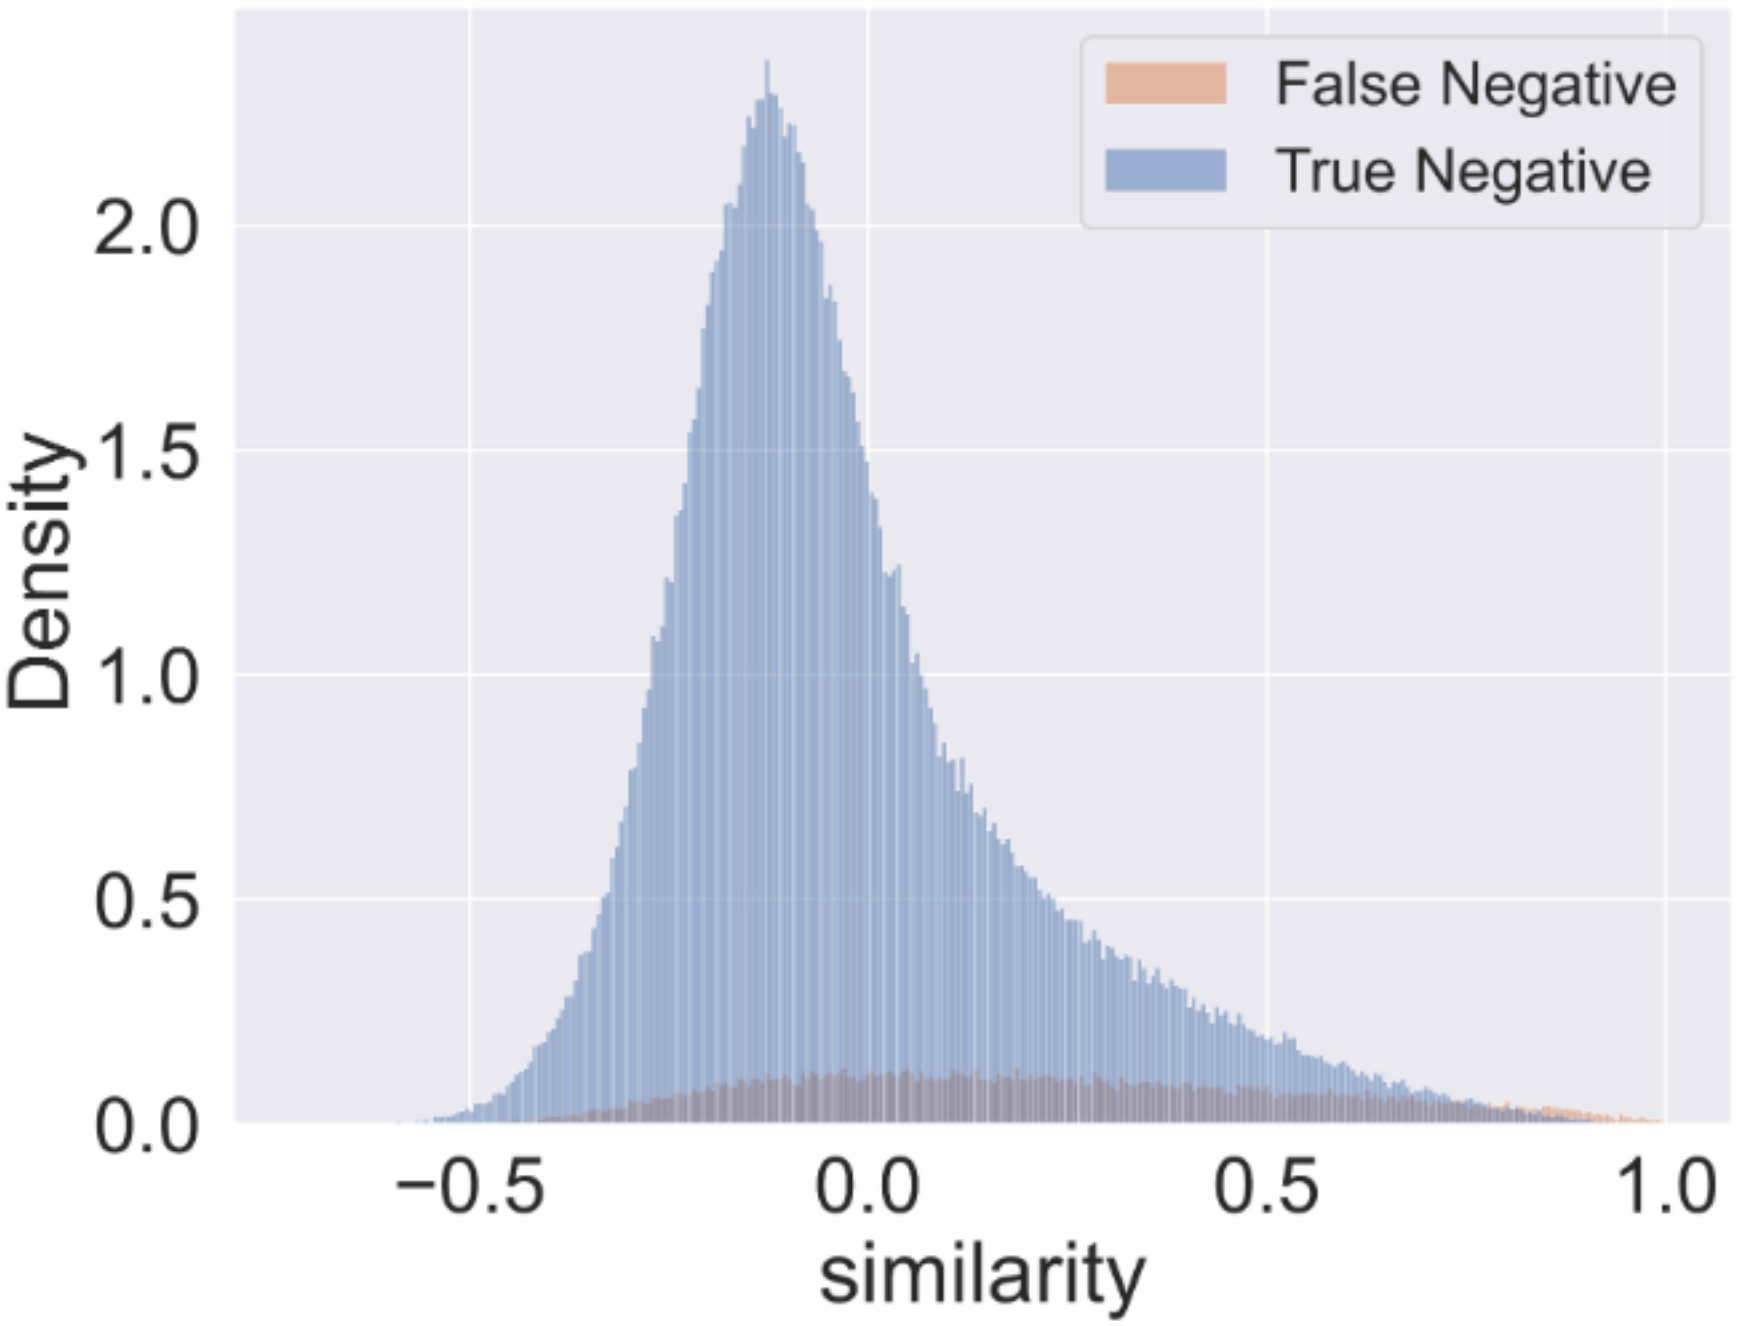
\includegraphics[width=4.8cm]{images/sim_negatives_image_data.png} }}%
    \qquad
    \subfloat[\centering Coauthor-CS (Graph). Most similar negative samples are \acp{fn}.]
    {{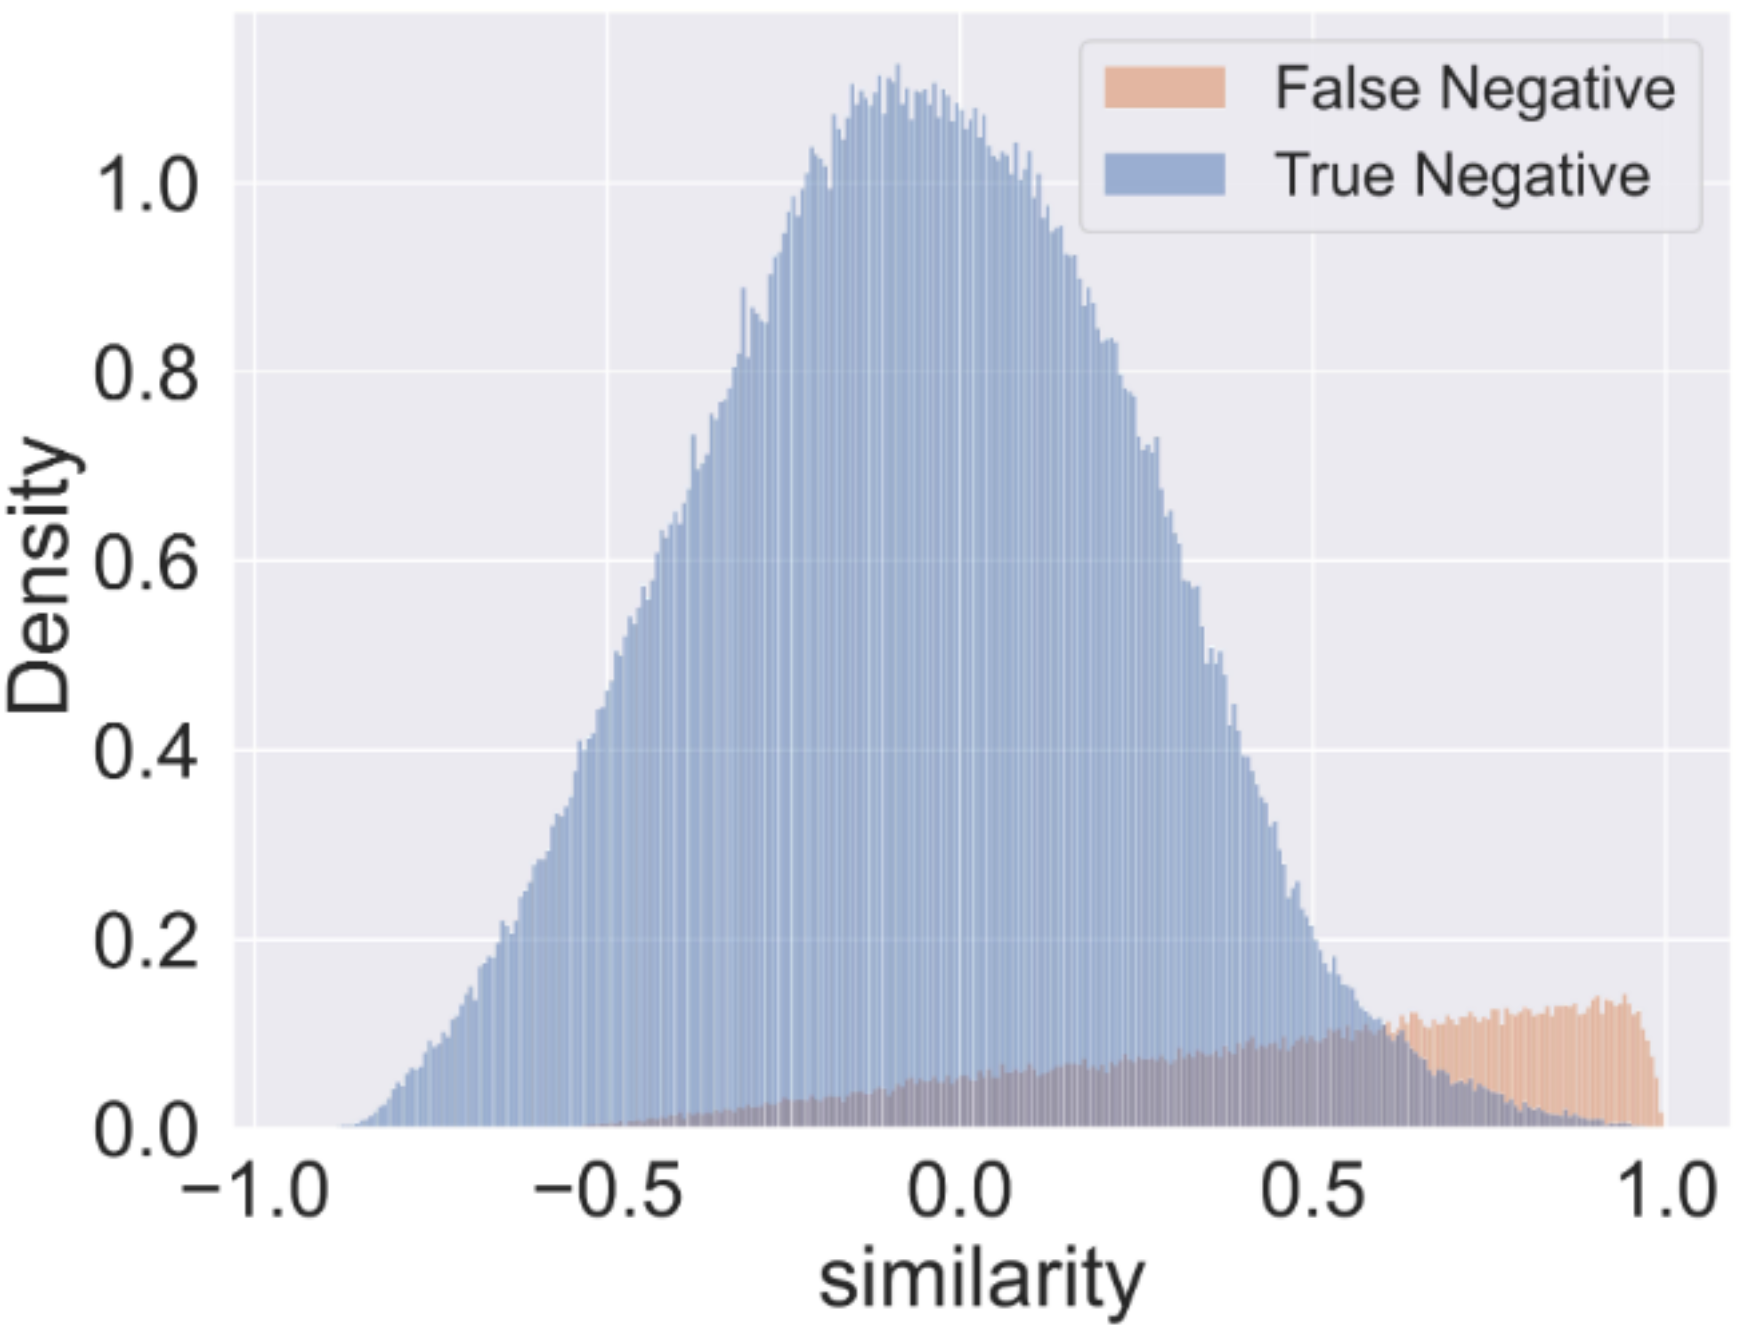
\includegraphics[width=5.2cm]{images/sim_negatives_graph_data.png} }}%
    \caption{Histogram of similarity between anchor and negative samples for \ac{cl} and \ac{gcl} from \citet{progcl_2022}.
    Blue denotes the empirical distribution of the \acp{tn}, while orange denotes \acp{fn}.}%
    \label{fig:sim_t_f_neg_image_graph}%
\end{figure}

% scheme 1: ProGCL-weight
Building on this observation, the authors propose incorporating both the probability of a sample being a \ac{tn} and 
the sample's similarity to the anchor, referred to as its hardness, into the negative sample selection process. 
It is important to note that the anchor is not a cluster center, 
but rather the sample from which augmentations are derived.

% scheme 2: ProGCL-mix (cf. MoCHi)
